\section{Aim}
 To study some more basic SQL queries like, SELECT DISTINCT, IN, ALTER TABLE, ORDER BY, etc.

\section{{Theory}}

\begin{itemize}
	\item SELECT DISTINCT: Used to remove duplicate rows from the output. 
	\item IN operator: Used to check if a given value is in a set of values.
	\item ALTER TABLE: Used to alter the properties of an existing table. 
	\item ORDER BY: Used to sort the output on a column. 
\end{itemize}

\section{{Code and Output}}

\begin{enumerate}
\item List the names of all companies as mentioned in the database\newline
\begin{minted}{sql}

SELECT DISTINCT company FROM car_details;

\end{minted}
\newline
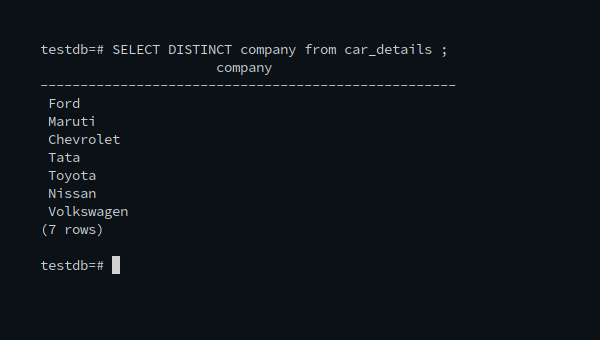
\includegraphics[width=\linewidth]{../Images/Basics/13.png}\newline
\item List the names of all countries having car production companies\newline
\begin{minted}{sql}

SELECT DISTINCT country FROM car_details;

\end{minted}
\newline
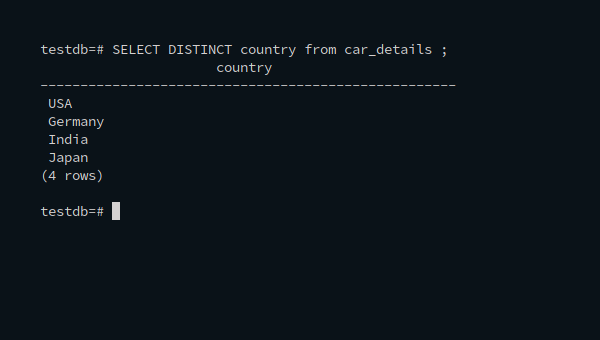
\includegraphics[width=\linewidth]{../Images/Basics/14.png}\newline
\item List the details of all cars within a price range 4 to 7 lakhs\newline
\begin{minted}{sql}

SELECT * FROM car_details 
	WHERE approxprice BETWEEN 4 AND 7; 

\end{minted}
\newline
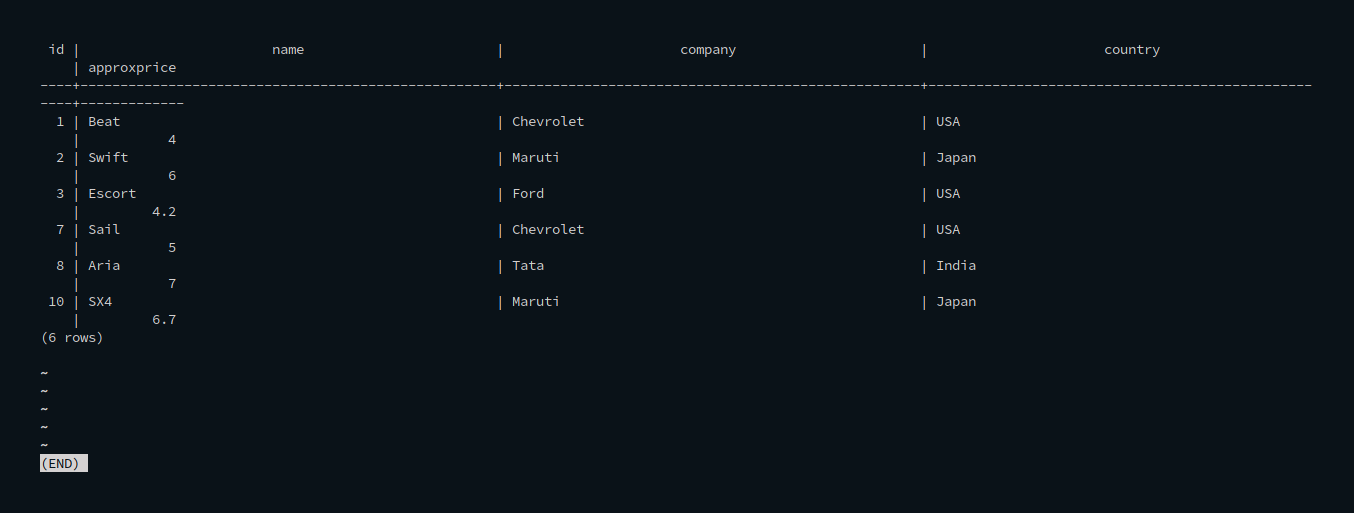
\includegraphics[width=\linewidth]{../Images/Basics/15.png}\newline
\item List the name and company of all cars originating from Japan and having price less than 6 lakhs\newline
\begin{minted}{sql}

SELECT name, company FROM car_details 
	WHERE country='Japan' AND approxprice <= 6;

\end{minted}
\newline
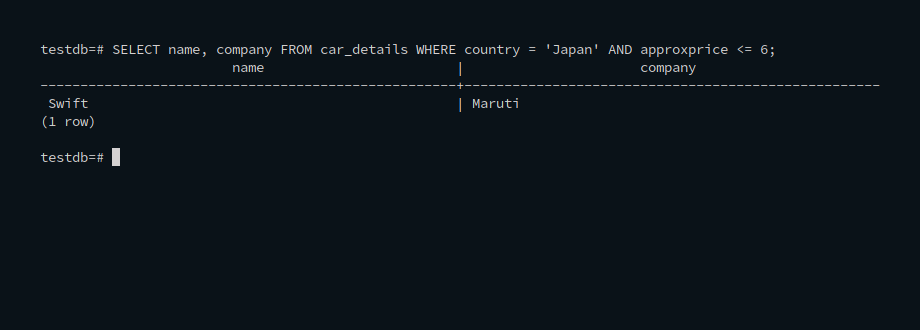
\includegraphics[width=\linewidth]{../Images/Basics/16.png}\newline
\item List the names and the companies of all cars either from Nissan or having a price greater than 20 lakhs.\newline
\begin{minted}{sql}

SELECT name, company FROM car_details 
	WHERE country='Nissan' AND approxprice >= 20;

\end{minted}
\newline
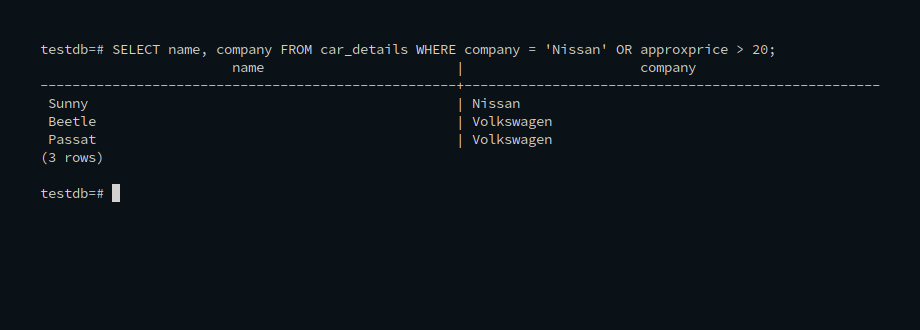
\includegraphics[width=\linewidth]{../Images/Basics/17.png}\newline
\item List the names of all cars produced by (Maruti,Ford).Use SQL IN statement.\newline
\begin{minted}{sql}

SELECT name FROM car_details 
	WHERE company IN ('Maruti', 'Ford');

\end{minted}
\newline
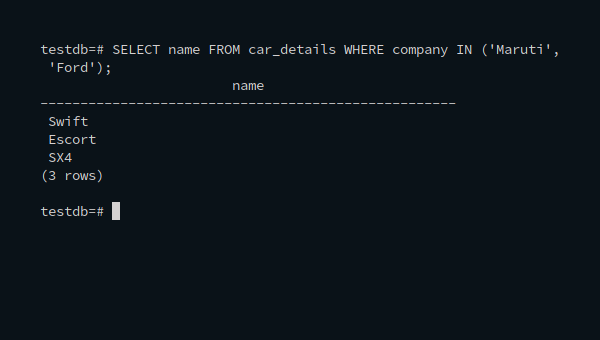
\includegraphics[width=\linewidth]{../Images/Basics/18.png}\newline
\item Alter the table cars to add a new field year (model release year).Upadate the year column for all the rows in the database.\newline
\begin{minted}{sql}

ALTER TABLE car_details ADD COLUMN year int;
UPDATE car_details SET year=2015;

\end{minted}
\newline
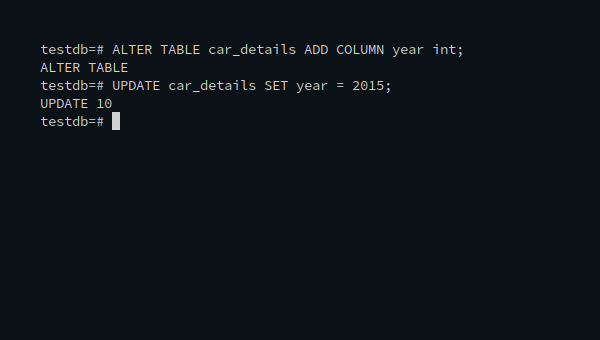
\includegraphics[width=\linewidth]{../Images/Basics/19.png}\newline
\item Display the names of all cars as Car\_name (while displaying the name attribute should be listed as car\_aliases)\newline
\begin{minted}{sql}

SELECT name as car_name FROM car_details;

\end{minted}
\newline
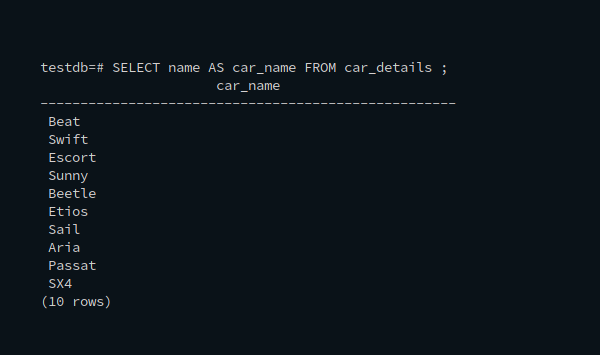
\includegraphics[width=\linewidth]{../Images/Basics/20.png}\newline
\item Rename the attribute name to car\_name\newline
\begin{minted}{sql}

ALTER TABLE car_details RENAME COLUMN name to car_name;

\end{minted}
\newline
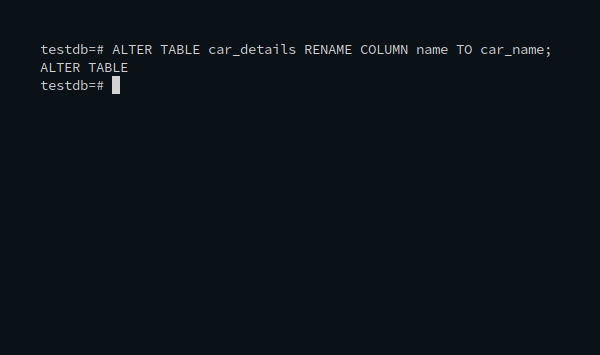
\includegraphics[width=\linewidth]{../Images/Basics/21.png}\newline
\item List the car manufactured by Toyota(to be displayed as cars\_Toyota)\newline
\begin{minted}{sql}

SELECT car_name as cars_toyota FROM car_details 
	WHERE company='Toyota';

\end{minted}
\newline
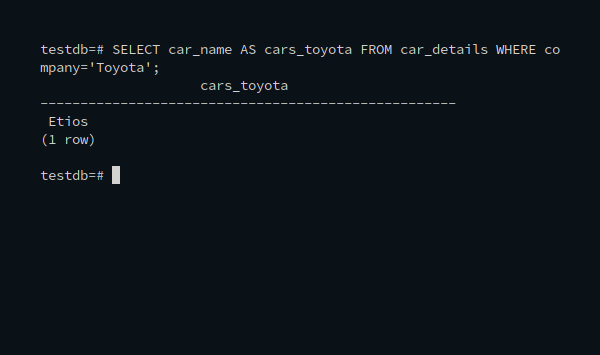
\includegraphics[width=\linewidth]{../Images/Basics/22.png}\newline
\item List the details of all cars in alphabetical order\newline
\begin{minted}{sql}

SELECT * FROM car_details ORDER BY car_name;

\end{minted}
\newline
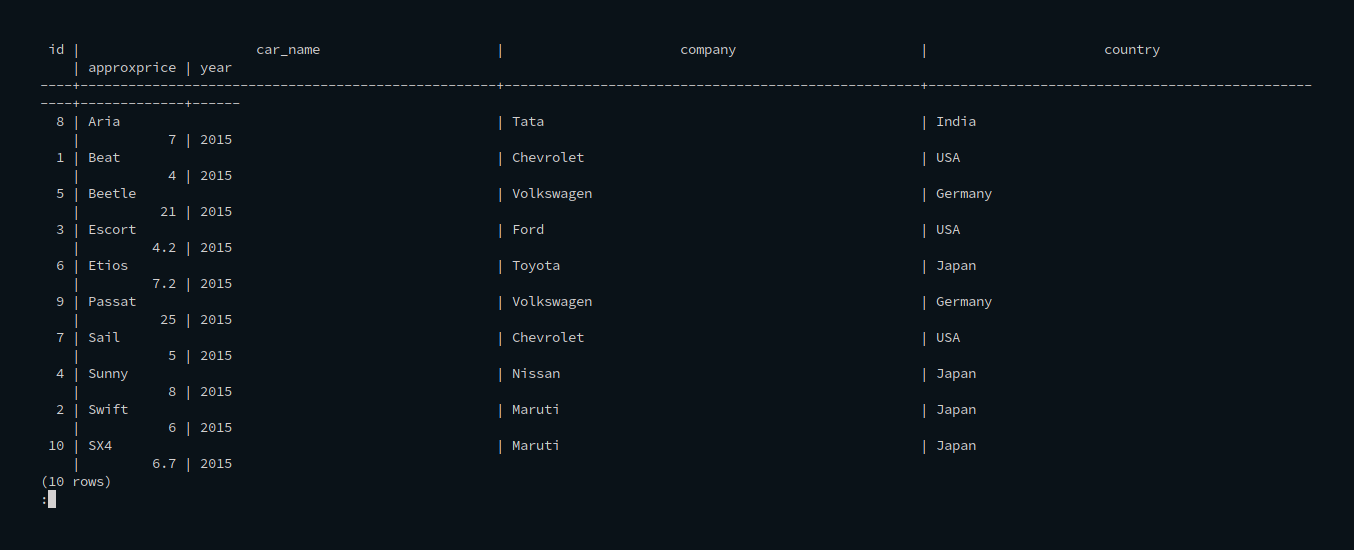
\includegraphics[width=\linewidth]{../Images/Basics/23.png}\newline
\item List the details of all cars from cheapest to costliest.\newline
\begin{minted}{sql}

SELECT * FROM car_details ORDER BY approxprice;

\end{minted}
\newline
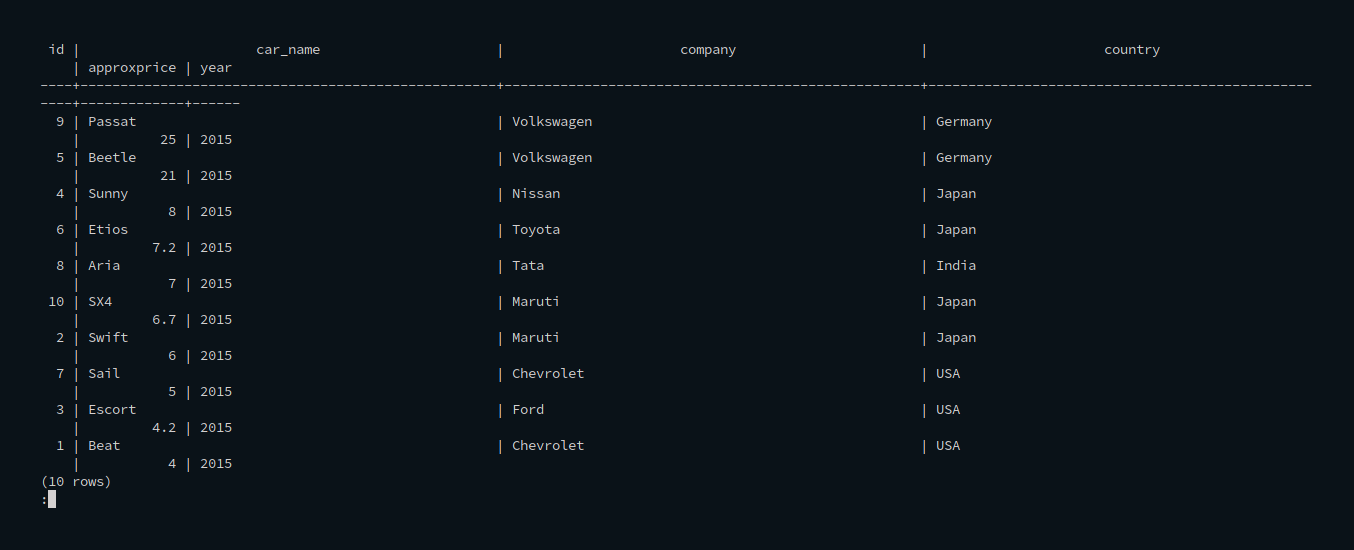
\includegraphics[width=\linewidth]{../Images/Basics/24.png}\newline
\end{enumerate}

\section{Result}
Implemented the program for Basic SQL Queries using Postgresql 11.5 on Manjaro Linux and the output was obtained.